\documentclass[journal,12pt,twocolumn]{IEEEtran}

\usepackage[utf8]{inputenc}
\usepackage{kvmap}
\usepackage{graphics} 

\usepackage{setspace}
\usepackage{gensymb}

\singlespacing

\usepackage{amsthm}

\usepackage{mathrsfs}
\usepackage{txfonts}
\usepackage{stfloats}
\usepackage{bm}
\usepackage{cite}
\usepackage{cases}
\usepackage{subfig}

\usepackage{longtable}
\usepackage{multirow}

\usepackage{enumitem}
\usepackage{mathtools}
\usepackage{steinmetz}
\usepackage{tikz}
\usepackage{circuitikz}
\usepackage{verbatim}
\usepackage{tfrupee}
\usepackage[breaklinks=true]{hyperref}
\usepackage{graphicx}
\usepackage{tkz-euclide}
\usepackage{float}

\usetikzlibrary{calc,math}
\usepackage{listings}
    \usepackage{color}                                            %%
    \usepackage{array}                                            %%
    \usepackage{longtable}                                        %%
    \usepackage{calc}                                             %%
    \usepackage{multirow}                                         %%
    \usepackage{hhline}                                           %%
    \usepackage{ifthen}                                           %%
    \usepackage{lscape}     
\usepackage{multicol}
\usepackage{chngcntr}

\DeclareMathOperator*{\Res}{Res}

\renewcommand\thesection{\arabic{section}}
\renewcommand\thesubsection{\thesection.\arabic{subsection}}
\renewcommand\thesubsubsection{\thesubsection.\arabic{subsubsection}}

\renewcommand\thesectiondis{\arabic{section}}
\renewcommand\thesubsectiondis{\thesectiondis.\arabic{subsection}}
\renewcommand\thesubsubsectiondis{\thesubsectiondis.\arabic{subsubsection}}

\hyphenation{op-tical net-works semi-conduc-tor}
\def\inputGnumericTable{}                                 %%

\lstset{
%language=C,
frame=single, 
breaklines=true,
columns=fullflexible
}
\begin{document}

\newtheorem{theorem}{Theorem}[section]
\newtheorem{problem}{Problem}
\newtheorem{proposition}{Proposition}[section]
\newtheorem{lemma}{Lemma}[section]
\newtheorem{corollary}[theorem]{Corollary}
\newtheorem{example}{Example}[section]
\newtheorem{definition}[problem]{Definition}

\newcommand{\BEQA}{\begin{eqnarray}}
\newcommand{\EEQA}{\end{eqnarray}}
\newcommand{\define}{\stackrel{\triangle}{=}}
\newcommand\hlight[1]{\tikz[overlay, remember picture,baseline=-\the\dimexpr\fontdimen22\textfont2\relax]\node[rectangle,fill=blue!50,rounded corners,fill opacity = 0.2,draw,thick,text opacity =1] {$#1$};}
\bibliographystyle{IEEEtran}
\providecommand{\mbf}{\mathbf}
\providecommand{\pr}[1]{\ensuremath{\Pr\left(#1\right)}}
\providecommand{\qfunc}[1]{\ensuremath{Q\left(#1\right)}}
\providecommand{\sbrak}[1]{\ensuremath{{}\left[#1\right]}}
\providecommand{\lsbrak}[1]{\ensuremath{{}\left[#1\right.}}
\providecommand{\rsbrak}[1]{\ensuremath{{}\left.#1\right]}}
\providecommand{\brak}[1]{\ensuremath{\left(#1\right)}}
\providecommand{\lbrak}[1]{\ensuremath{\left(#1\right.}}
\providecommand{\rbrak}[1]{\ensuremath{\left.#1\right)}}
\providecommand{\cbrak}[1]{\ensuremath{\left\{#1\right\}}}
\providecommand{\lcbrak}[1]{\ensuremath{\left\{#1\right.}}
\providecommand{\rcbrak}[1]{\ensuremath{\left.#1\right\}}}
\theoremstyle{remark}
\newtheorem{rem}{Remark}
\newcommand{\sgn}{\mathop{\mathrm{sgn}}}
\providecommand{\abs}[1]{\left\vert#1\right\vert}
\providecommand{\res}[1]{\Res\displaylimits_{#1}} 
\providecommand{\norm}[1]{$\left\lVert#1\right\rVert$}
%\providecommand{\norm}[1]{\lVert#1\rVert}
\providecommand{\mtx}[1]{\mathbf{#1}}
\providecommand{\mean}[1]{E\left[ #1 \right]}
\providecommand{\fourier}{\overset{\mathcal{F}}{ \rightleftharpoons}}
%\providecommand{\hilbert}{\overset{\mathcal{H}}{ \rightleftharpoons}}
\providecommand{\system}{\overset{\mathcal{H}}{ \longleftrightarrow}}
	%\newcommand{\solution}[2]{\textbf{Solution:}{#1}}
\newcommand{\solution}{\noindent \textbf{Solution: }}
\newcommand{\cosec}{\,\text{cosec}\,}
\providecommand{\dec}[2]{\ensuremath{\overset{#1}{\underset{#2}{\gtrless}}}}
\newcommand{\myvec}[1]{\ensuremath{\begin{pmatrix}#1\end{pmatrix}}}
\newcommand{\mydet}[1]{\ensuremath{\begin{vmatrix}#1\end{vmatrix}}}
\numberwithin{equation}{subsection}
\makeatletter
\@addtoreset{figure}{problem}
\makeatother
\let\StandardTheFigure\thefigure
\let\vec\mathbf
\renewcommand{\thefigure}{\theproblem}
\def\putbox#1#2#3{\makebox[0in][l]{\makebox[#1][l]{}\raisebox{\baselineskip}[0in][0in]{\raisebox{#2}[0in][0in]{#3}}}}
     \def\rightbox#1{\makebox[0in][r]{#1}}
     \def\centbox#1{\makebox[0in]{#1}}
     \def\topbox#1{\raisebox{-\baselineskip}[0in][0in]{#1}}
     \def\midbox#1{\raisebox{-0.5\baselineskip}[0in][0in]{#1}}
\vspace{3cm}
\title{\textbf{Matrices Assignment - Conic} }
\author{Dukkipati Vijay Sai}
\maketitle
\newpage
\bigskip
\renewcommand{\thefigure}{\theenumi}
\renewcommand{\thetable}{\theenumi}
Get Python code for the figure from 
\begin{lstlisting}
https://github.com/dukkipativijay/Fwciith2022/tree/main/Assignment%201/Codes/src
\end{lstlisting}
Get LaTex code from
\begin{lstlisting}
https://github.com/dukkipativijay/Fwciith2022/tree/main/Assignment%201%20-%20Assembly/Codes
\end{lstlisting}
%
\section{Question}
\centering
\textbf{\textit{Class 12-1, Exercise 6.3,Q(27)}}\\
\vspace{0.25cm}
\raggedright
\textbf{The line $y = x + 1$ is a tangent to the curve $y^2 = 4x$ at the point?} \\
\centering
\vspace{0.25cm}
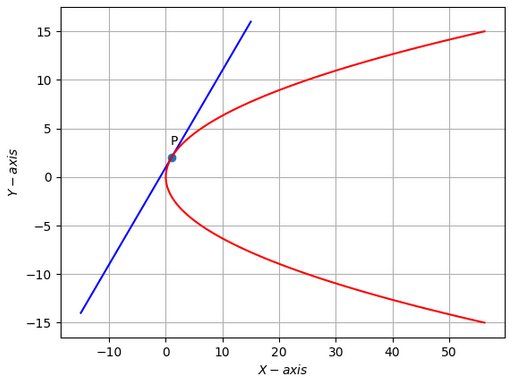
\includegraphics[width=0.5\textwidth]{conicfig.png}
Figure 1 - Conic with Tangent at P

\section{Construction}
\vspace{0.25cm}
\raggedright
\centering
\begin{tabular}{|c|c|c|}
\hline
\textbf{Symbol} & \textbf{Value} & \textbf{Description}\\
\hline
L & $ y = x + 1 $ & Line L\\
\hline
C & $ y^2 = 4x$ & Conic C\\
\hline
P & $ x_i = q + \mu_i m$ & Point of Contact P\\
\hline
\end{tabular}\\
\vspace{0.2cm}
\centerline{Table 1: Parameters Table}
\section{Solution}
\raggedright
Let P be the point of Contact of the Line $y = x + 1$ to the parabola  $y^2 = 4x$\\

\vspace{0.25cm}


The point of intersection of line\\
\vspace{0.25cm}
\centering
$L : \vec{x} = \vec{q} + \mu \vec{m}  \hspace{0.4cm} \mu \epsilon \mathbb{R} \hspace{1cm} (1)$\\
\vspace{0.25cm}
\raggedright
With the conic section\\
\vspace{0.25cm}
\centering
$ \vec{x}^T \vec{V}\vec{x} + 2 \vec{u}^T \vec{x} + f = 0 \hspace{1cm} (2)$\\
\vspace{0.25cm}
\raggedright
is given by\\
\vspace{0.25cm}
\centering
$ \vec{x}_i = \vec{q} + \mu_i \vec{m} \hspace{2.5cm} (3)$ \\
\vspace{0.25cm}
\raggedright
Where\\
\vspace{0.25cm}
$\mu_i = \frac{1}{\vec{m^T Vm}}(-\vec{m^T(Vq+u)} \pm \sqrt{[\vec{m^T(Vqu})]^2 - (\vec{q}^T \vec{Vq} + 2 \vec{u^T q} + f) (\vec{m^T Vm})}$ ) \hspace{0.1cm} (4) \\
\vspace{0.25cm}
\raggedright
If the line L touches the conic at exactly one point,the conic intercept has exactly one root. Hence, \\
\vspace{0.25cm}
\centering
$ [\vec{m^T(Vqu})]^2 - (\vec{m^T Vm}) (\vec{q}^T \vec{Vq} + 2 \vec{u^T q} + f)  = 0$ (5)\\
\vspace{0.25cm}
\raggedright
The equation of our Conic (which here is a parabola) is,\\
\vspace{0.25cm}
\centering 
$y^2 = 4x$ \hspace{2.2cm}(6) \\
\vspace{0.4cm}
\raggedright
Comparing it with the General Equation of a Conic,\\
\vspace{0.25cm}
\centering
$Ax^2 + Bxy + Cy^2 + Fx + Gy + f = 0$ \hspace{0.5cm}(7)\\
\vspace{0.25cm}
\raggedright
We Have,\\
\vspace{0.25cm}
A = 0, B = 0, C = 1, F = -4, G = 0, f = 0\\
\vspace{0.25cm}
We Know That,\\
\vspace{0.25cm}
\centering
$ V = \myvec{A&\frac{B}{2}\\\\\frac{B}{2}&C} \hspace{2cm} u = \myvec{\frac{F}{2}\\\\\frac{G}{2}} $\\
\vspace{0.25cm}
\raggedright
So we get,\\
\vspace{0.25cm}
\centering
$ V = \myvec{0&0\\0&1} \hspace{2.2cm} u = \myvec{-2\\0} $ \\
\vspace{0.25cm}
\raggedright
Hence, the Eq. (6) of our Parabola can be written in the form of Conic Eq. (2) as,\\
\vspace{0.25cm}
\centering
$\vec{x^T} \myvec{0&0\\0&1}\vec{x} + 2 \myvec{-2&0} \vec{x} + 0 = 0$ \hspace{0.5cm} (8)\\ 
\vspace{0.25cm}
\raggedright
Let us consider the direction vector of \textbf{L} as m,\\
\vspace{0.25cm}
\centering
$ \vec{m} = \myvec{1\\ \lambda}$ \hspace{1cm} (9)\\
\vspace{0.25cm}
\raggedright
and \textbf{q} be any point on the Line $y = x + 1$,\\
\vspace{0.25cm}
\centering
$ \vec{q} = \myvec{0\\1}$ \hspace{1cm} (10)\\
\vspace{0.25cm}
\raggedright
The Equation of the given line can be re-written as,\\
\vspace{0.25cm}
\centering
$ x - y = -1 $\\
\vspace{0.25cm}
\raggedright
Comparing it with the normal form of the line,\\
\vspace{0.25cm}
\centering
$ \vec{n}^T \vec{x} = c $ \\
\vspace{0.25cm}
\raggedright
We Get,\\
\vspace{0.25cm}
\centering
$ \vec{n}^T = \myvec{1&-1} \hspace{0.2cm} and \hspace{0.2cm} c = -1$\\
\vspace{0.25cm}
\raggedright
Hence,\\
\vspace{0.25cm}
\centering
$ m = \myvec{1 \\ 1} $ \\
\vspace{0.25cm}
\raggedright
From Eq. (4) and (5)\\
\vspace{0.25cm}
\centering
$ \mu_i = \frac{1}{\vec{m^T Vm}} ( - \vec{m^T (Vq + u)})$\\
\vspace{0.25cm}
$ \mu_i = \frac{1}{\myvec{1 & 1} \myvec{0&0\\0&1} \myvec{1\\1}} ( - \myvec{1&1} ( \myvec{0&0\\0&1} \myvec{0\\1} + \myvec{-2\\0})$\\ 
\vspace{0.25cm}
$ \mu_i = \frac{1}{\myvec{0 & 1} \myvec{1\\1}} ( - \myvec{1&1} ( \myvec{0\\1} + \myvec{-2\\0})$\\ 
\vspace{0.25cm}
$ \mu_i = \frac{1}{1} ( - \myvec{1&1} ( \myvec{-2\\1} )$\\ 
\vspace{0.25cm}
$ \mu_i = 1$\\ 
\vspace{0.4cm}
\raggedright
Now Eq. (3) becomes,\\
\vspace{0.25cm}
\centering
$ \myvec{x \\ y} = \myvec{0\\1} + (1)  \myvec{1 \\ 1} $ \\
\vspace{0.25cm}
$ \myvec{x \\y } = \myvec{0\\1} + \myvec{1\\1} $ \\
\vspace{0.25cm}
$ \myvec{x \\y } = \myvec{1\\2} $ \\

\raggedright
Therefore,\\

\centering
$ P = \myvec{1\\2}$ \\

\raggedright
Is the required point of contact of the given line and the conic.
\end{document}
Footer